% manuscript produces a one-column, double-spaced document:
%\documentclass[12pt,preprint]{aastex}
\documentclass[twocolumn]{aastex6}
%\documentclass[iop]{emulateapj}

% preprint2 produces a double-column, single-spaced document:
%\documentclass[preprint2]{aastex}

%Packages
%\usepackage[colorlinks=true,linkcolor=blue,citecolor=blue]{hyperref}

\usepackage{natbib}
\usepackage[caption=false]{subfig}
\usepackage{amsmath,amssymb}
\newcommand{\vdag}{(v)^\dagger}
\newcommand{\degree}{$^\circ$}
\newcommand{\vtan}{$V_{tan}$}
\newcommand{\kms}{km~s$^{-1}$}
\newcommand{\msun}{M$_{\sun}$}
\newcommand{\rjup}{R$_{Jup}$}
\newcommand{\ldl}{$\lambda/{\Delta}{\lambda}$}
\newcommand{\lsun}{L$_{\sun}$}
\newcommand{\lbol}{$\log_{10}{L_{bol}/L_{\sun}}$}
\newcommand{\teff}{T$_{eff}$}
\newcommand{\logg}{$\log{g}$}
\newcommand{\fsed}{$f_{sed}$}
\newcommand{\kzz}{$K_{zz}$}
\newcommand{\meth}{CH$_4$}
\newcommand{\wat}{H$_2$O}
\newcommand{\sha}{2MASS~J0835$-$0819}
\newcommand{\shb}{2MASS~J1821+1414}

\slugcomment{To be submitted to ApJ/AJ}


\shorttitle{Spectral Variability of L Dwarfs}
\shortauthors{Schlawin et al.}


\begin{document}


\title{Spectral Variability of Two Rapidly Rotating Brown Dwarfs: \\2MASS~J08354256$-$0819237 and 2MASS~J18212815+1414010}

%% Use \author, \affil, and the \and command to format
%% author and affiliation information.
%% Note that \email has replaced the old \authoremail command
%% from AASTeX v4.0. You can use \email to mark an email address
%% anywhere in the paper, not just in the front matter.
%% As in the title, use \\ to force line breaks.

\author{E. Schlawin\altaffilmark{1,2}, Adam J.\ Burgasser\altaffilmark{2,3}, J. Gizis\altaffilmark{4}, T. Karalidi\altaffilmark{1}, \and J. Teske\altaffilmark{5}}

\altaffiltext{1}{Steward Observatory, Tucson AZ 85721 \email{eas342@email.arizona.edu}}
\altaffiltext{2}{Visiting Astronomer at the Infrared Telescope Facility, which is operated by the University of Hawaii under contract NNH14CK55B with the National Aeronautics and Space Administration}
\altaffiltext{3}{Center for Astrophysics and Space Science, University of California San Diego, La Jolla, CA 92093, USA}
\altaffiltext{4}{Department of Physics and Astronomy, University of Delaware, Newark, DE 19716, USA}
\altaffiltext{5}{Carnegie Observatories, 813 Santa Barbara Street, Pasadena, CA 91101, USA}

\begin{abstract}
Low-temperature L dwarfs exhibit low-level, rotationally-modulated photometric variability generally associated with heterogeneous, cloud-covered atmospheres. The spectral character of these variations yield insight into the particle sizes and vertical structure of the clouds. Here we present the results of a high precision, ground-based, near-infrared, spectral monitoring study of two mid-type L dwarfs, 2MASS~J08354256$-$0819237 and 2MASS~J18212815+1414010, using the SpeX instrument on the Infrared Telescope Facility. By simultaneously observing a nearby visual companion, we achieve $<$0.15\% per-band sensitivity in relative brightness changes across the 0.9--2.4$\mu$m bandwidth. We find that 2MASS~J0835$-$0819 exhibits marginal ($\lesssim$ 0.5\% per band) variability with no spectral dependence while 2MASS~J1821+1414 varies by up to $\pm$1.3\% at 0.9~$\mu$m, with the variability amplitude declining toward longer wavelengths.  {\bf [PHASE VARIATION]}. The latter result extends the variability trend observed in prior $HST$/WFC3 spectral monitoring of 2MASS~J1821+1414, and we show that the full 1--2.5~$\mu$m variability amplitude spectrum can be reproduced by Mie extinction of sub-micron dust particles, although this model becomes too strong at short wavelengths. An alternate model based on surface hot spots requires implausibly large temperature variations. The different variability behaviors of 2MASS~J0835$-$0819 and  2MASS~J1821+1414 suggests dependencies on viewing angle and/or overall cloud content, underlying factors that can be examined through a broader variability survey.
\end{abstract}


\keywords{techniques: spectroscopic -- stars: atmospheres -- stars: brown dwarfs -- stars: individual (\objectname{2MASS J08354256-0819237}, \objectname{2MASS J18212815+1414010}) -- stars: late-type -- stars: variables: general}



\section{Introduction}

The atmospheres of L-type stars and brown dwarfs (1300~K $\lesssim$ {\teff} $\lesssim$ 2200~K; \citealt{2015ApJ...810..158F}) are sufficiently cool that species of mineral and metal condensates form spontaneously in their atmospheres \citep{1996A&A...305L...1T,2010ApJ...716.1060V}.
In addition to influencing spectral energy distributions (e.g., \citealt{2001ApJ...556..357A,2008ApJ...674..451B}) and photospheric chemistry (e.g., \citealt{2000ApJ...531..438B}), condensates can coalesce into large-scale cloud and haze structures \citep{1989ApJ...338..314L,2001ApJ...556..872A,2014Natur.505..654C}
whose surface and vertical structure may produce rotationally-modulated brightness variations (e.g., \citealt{2012ApJ...750..105R}), and long-term variations from differential rotation and/or cloud structure evolution (e.g., \citealt{2009ApJ...701.1534A,2013A&A...555L...5G,2016ApJ...826....8Y}). Evidence of cloud-driven variability extends to the cooler T dwarfs (e.g., \citealt{2009ApJ...701.1534A,2012ApJ...760L..31B,2015ApJ...799..154M}), and virtually all L dwarfs and most T dwarfs likely have cloud deck heterogeneities leading to infrared flux variations $\gtrsim$0.2\% in amplitude \citep{2015ApJ...799..154M}. Clouds and hazes are important constituents of exoplanetary atmospheres as well (e.g., \citealt{2011ApJ...733...65B,2014Natur.505...69K,2016Natur.529...59S}).

Multi-wavelength monitoring of low-temperature stars and brown dwarfs allows the measurement of cloud vertical structure and composition, as gray grain scattering opacity competes with strongly wavelength-dependent molecular gas opacity. The amplitude of variability as a function of wavelength samples the vertical depths of cloud layers \citep{2013ApJ...768..121A}, and amplitude spectra have been shown to vary with effective temperature, ({\teff}; e.g., \citealt{2015ApJ...798L..13Y}) and surface gravity (e.g., \citealt{2016ApJ...829L..32L}).
Wavelength-dependent phase variance in lightcurves has also been observed \citep{2012ApJ...760L..31B,2013ApJ...778L..10B,2016ApJ...826....8Y}.
Since different wavelengths sample different photospheric depths in the highly structured spectra of L and T dwarfs, these phase variations have been interpreted as arising from the relative motion of distinct cloud layers or deep thermal pulsation \citep{2014ApJ...785..158R}. 

Broad-band variability amplitudes are typically $<$1\% in L and T dwarfs, with some dramatic exceptions \citep{2009ApJ...701.1534A,2012ApJ...750..105R,2013A&A...555L...5G,2016ApJ...829L..32L}. 
Ground-based spectral (e.g., CLOUDS; \citealt{2008A&A...487..277G}) and broad-band photometric monitoring surveys (e.g., \citealt{1999A&A...348..800B,2003MNRAS.346..473K,2014ApJ...793...75R,2014A&A...566A.111W}) are generally limited to $>$1-3\% relative precision due to telluric atmospheric instabilities (i.e., ``red noise'') and insufficient calibrators \citep{2003MNRAS.339..477B}.
In contrast, the stability of space-based platforms such as $Hubble$ $Space$ $Telescope$ ($HST$), $Spitzer$ and $Kepler$ provide order-of-magnitude improvements in relative photometric and spectro-photometric precision, and have been responsible for the discovery of the majority of known L and T dwarf variables \citep{2013ApJ...768..121A,2013ApJ...779..172G,2015ApJ...799..154M}. However, these facilities are poorly suited for building up robust statistical samples to assess the physical origins of surface heterogeneity, or evolution in variability modes. 

Ground-based Multi-Object Spectroscopy (MOS) with a multi-object or long slit spectrograph, in which references stars are simultaneously observed to correct for telluric effects  (e.g., \citealt{bean10,bean2013,gibson13clouds,stevenson2016hatp26}) can significantly improve the precision of ground-based spectro-photometry. \citet{2014ApJ...783....5S} achieved $<$0.1\% per band variability precision for the planet-host star Corot-1 using the NASA Infrared Telescope Facility (IRTF) SpeX spectrograph \citep{2003PASP..115..362R}, by simultaneously monitoring the star and a nearby visual binary companion in a wide (3$\arcsec$) slit. This was sufficient to infer the presence of a cloud/haze layer in Corot-1b via transmission spectroscopy. A similar investigation of the disintegrating rocky exoplanet KIC 12557548b  enabled the characterization of the grain properties of its tidal debris tail \citep{2016ApJ...826..156S}. In a parallel effort, \citet{2014ApJ...785...48B} obtained $<$0.5\% per-band relative precision across the 1--2.5~$\mu$m band with IRTF/SpeX for the variable T dwarf Luhman 16B, by simultaneously observing it and its L dwarf companion. These studies demonstrate that high-precision, near-infrared spectral monitoring observations can be achieved from the ground.

\begin{deluxetable*}{lllcccccccl}
\tablecaption{Brown Dwarf Properties}\label{tab:bdProp}
\tablewidth{0pt}
\tablehead{
 & \multicolumn{2}{c}{Spectral Type} \\
\colhead{Name} & 
\colhead{Opt} & 
\colhead{NIR} & 
\colhead{$d$} & 
\colhead{2MASS $H$} & 
\colhead{$J-K_s$} & 
\colhead{\teff} & 
\colhead{P$_{rot}$} &
\colhead{$v\sin{i}$} & 
\colhead{$i$\tablenotemark{a}} & 
\colhead{Refs} \\
 &  &  & \colhead{(pc)} & &  & \colhead{(K)} & \colhead{(hr)} & \colhead{(km/s)} & \colhead{($\degr$)} \\
 }
\startdata
\sha\ & L5 & L7 & 8.52$\pm$0.08 & 11.94$\pm$0.02 & 2.03$\pm$0.03 & 1754$\pm$112 & 3.1\tablenotemark{b} & 14.18$\pm$0.43 & 21 & 1-5 \\
\shb\ & L4.5p & L5 & 9.38$\pm$0.03 & 12.40$\pm$0.02 & 1.78$\pm$0.03 & 1614$\pm$100\tablenotemark{c} & 4.2$\pm$0.1 & 28.85$\pm$0.16 & 83 & 5-10 \\
\enddata
\tablenotetext{a}{Estimated inclination angle $i$ assuming a radius = 1 Jupiter radius, so that $\sin{i}$ = 8.2$\times$10$^{-3}Pv\sin{i}$, where $P$ is in hours and $v\sin{i}$ is in km/s. A value of $i$ $\approx$ 0{\degree} is viewed pole-on, $i$ $\approx$ 90{\degree} is viewed equator-on.}
\tablenotetext{b}{Tentative period.}
\tablenotetext{c}{Estimated from the \citet{2015ApJ...810..158F} {\teff}/spectral type relation.}
\tablerefs{(1) \citet{2003AJ....126.2421C};
(2) \citet{2012ApJ...752...56F}; 
(3) \citet{2015ApJ...810..158F};
(4) \citet{2004MNRAS.354..378K};
(5) \citet{2010ApJ...723..684B};
(6) \citet{2008ApJ...686..528L}; 
(7) \citet{2016MNRAS.455..357S};
(8) \citet{2015ApJ...798...73G};
(9) \citet{2015ApJ...799..154M}
(10) \citet{2015ApJ...798L..13Y}; 
}
\end{deluxetable*}



\begin{figure*}
\centering
	\plottwo{image0835-0819.pdf}{image1821+1414.pdf}
	\label{fig:image1821}
	\vspace{-.9in}
	\caption{2MASS $JHK_s$ three-color images of the fields around our targets {\sha} (left) and {\shb} (right).  Each image is centered on the target, and span a 1$\arcmin\times\arcmin$ field of view oriented with North up and East the left. The comparison stars referred to in the text appear as blue sources in these images. }
	\label{fig:images}
	\vspace{0.17in}
\end{figure*} 

This article reports the results of a pilot study adapting these methods to measuring the variability of two L-type dwarfs with nearby visual companions. We describe our target selection process and pilot target properties in Section~\ref{sec:targets}.
In Section~\ref{sec:obs}, we describe our monitoring observations and data reduction procedures to generate relative spectro-photometric time series.
In Section~\ref{sec:analysis}, we analyze these time series using sinusoidal model fits over discrete spectral bands to generate individual light curves and amplitude spectra.
We then fit the variability amplitude spectra to two different physical models, Mie scattering from clouds and heterogeneous temperature spots, to assess which more accurately reproduces the data.
We summarize our results in Section~\ref{sec:conclusions}.


\section{Target Selection and Characterization}\label{sec:targets}

We identified potential targets for relative spectro-photometry by selecting among the $\approx$200 known L dwarfs\footnote{We identified these sources from DwarfArchives,  \url{http://dwarfarchives.org}. The declination range corresponds to the visibility region of IRTF.} with $H$ $<$ 14 and $-$30{\degree}  $<$ $\delta$ $<$ +67{\degree} those sources that have comparable-brightness ($\Delta{H}$ $<$ 1) visual binary companions at apparent separations of 5$\arcsec$--30$\arcsec$. We identified 30 potential targets, and prioritized those with previously detected photometric variability or rotational $v\sin{i}$ measurements indicating periods $\leq$10~hr.  Two sources were identified as ideal initial targets (Table~\ref{tab:bdProp}).

2MASS~J08354256$-$0819237 (hereafter {\sha}; \citealt{2003AJ....126.2421C} is a bright, nearby ($d$ = 8.5$\pm$0.8~pc; \citealt{2012ApJ...752...56F}) L5 dwarf that shows signatures of low surface gravity \citep{2016ApJ...833...96L}. 
This source has been reported to vary in both optical and near-infrared bands with a period of 3.1~hr and an amplitude of $\sim$1\%  \citep{2004MNRAS.354..378K,2014A&A...566A.111W}.
Its $v\sin{i}$ = 14.2$\pm$0.4~{\kms} \citep{2010ApJ...723..684B} suggests a near pole-on viewing angle assuming a radius R = 1~{\rjup}.
There is an $H$ = 12.3 source (2MASS~J08354383$-$0819212) at a separation of 19$\arcsec$ suitable for relative flux calibration (Figure~\ref{fig:images}). 
2MASS J18212815+1414010 (hereafter {\shb}; \citealt{2008ApJ...686..528L}) is a similarly bright and nearby ($d$ = 9.38$\pm$0.03; \citealt{2016MNRAS.455..357S}) L4.5 dwarf, which exhibits a peculiar near-infrared spectrum attributed to youth and/or thick clouds \citep{2008ApJ...686..528L,2015ApJS..219...33G,2016ApJ...833...96L}.
This source is a photometric variable with a period of 4.2$\pm$0.1~hr \citep{2015ApJ...799..154M} and $v\sin{i}$ = 28.85$\pm$0.16~{\kms}, suggesting a near equator-on orientation.  \citet{2015ApJ...798L..13Y} measured 1--3\% spectral variability with $HST$/WFC3 over 1.1--1.6~$\micron$, with greater variabilty at shorter wavelengths.
There are two suitably bright comparison stars within 20$\arcsec$ for relative calibration: 2MASS~J18212812+1414089 with $H$ = 12.6 at 7$\arcsec$ separation and 2MASS~J18212715+1413482 with $H$ = 12.0 at 29$\arcsec$ separation; we chose the latter for our monitoring observations.



To characterize the atmospheric regions probed by our observations, we analyzed previously 
obtained IRTF/SpeX data for these sources \citep{2008ApJ...686..528L,2010ApJ...710.1142B}.
Direct comparison to spectral standards following the convention of \citet{2010ApJS..190..100K} indicate near-infrared
classifications of L7 for {\sha} and L5 for {\shb} (Figure~\ref{fig:tbright}). The former is considerably later than the L5 optical classification previously reported by \citet{2003AJ....126.2421C}. We confirm the intermediate low surface gravity classification (INT-G) reported by \citet{2016ApJ...833...96L} based on the indices of \citet{2013ApJ...772...79A} using an L7 classification. The discrepancy between the optical and near-infrared classifications of this source is likely related to surface gravity effects. {\shb}, on the other hand, is a good match to the L5 spectral standard and has a field dwarf gravity classification.

We computed brightness temperature spectra from these data as
\begin{equation}
T_{\lambda,surf} = \frac{hc}{k\lambda}\left[\ln\left(1+\frac{2\pi{hc^2}}{I_{\lambda,surf}\lambda^5}\right)\right]^{-1}
\end{equation}
where the surface flux density $I_{\lambda,surf}$ is computed as
\begin{equation}
I_{\lambda,surf} = {\pi}B_{\lambda} = I_{\lambda,obs}\left(\frac{d}{R}\right)^2 = I_{\lambda,abs}\left(\frac{10~{\rm pc}}{R}\right)^2
\end{equation}
$I_{\lambda,obs}$ and $I_{\lambda,abs}$ are the observed and absolute flux densities, $d$ the source distance and $R$ the source radius.  Both spectra were normalized to absolute flux densities using their 2MASS $H$ magnitudes and measured parallaxes \citep{2016MNRAS.455..357S,2016AJ....152...24W}. We adopted radii from the evolutionary models of \citet{2003A&A...402..701B} assuming effective temperatures ({\teff}s) from \citet{2015ApJ...810..158F} based on these sources' bolometric luminosity measurements (Table~\ref{tab:bdProp}). Uncertainties in the spectral fluxes, absolute photometric calibration, adopted {\teff} and radius were propagated by Monte Carlo simulation.  For {\sha} we considered two cases: radii corresponding to an age of 50--200~Myr, the age range estimated for INT-G sources by \citet{2013ApJ...772...79A}, for which the evolutionary models predict radii of 0.147~R$_{\odot}$ to 0.115~R$_{\odot}$; and an age range of 1--5~Gyr for which the evolutionary models predict radii of 0.092~R$_{\odot}$ to 0.084~R$_{\odot}$.
For {\shb}, we assumed a lower age limit of 200~Myr based on its FLD-G classification, and an upper limit of 700~Myr based on the analysis of \citet{2016MNRAS.455..357S} range of 1--5~Gyr; evolutionary models predict radii of 0.120~R$_{\odot}$ to 0.097~R$_{\odot}$ for these ages.  

Figure~\ref{fig:tbright} shows the resulting brightness temperature spectra and their uncertainties from these calculations.  The spectral peaks for {\sha} are roughly constant at {\teff} = 1900$\pm$50~K in the field surface gravity case, and declines from 1700$\pm$20~K at the $J$-band peak to 1570$\pm$60~K at the $K$-band peak in the low surface gravity case.
{\bf [Adam, Are these Numbers still true? Also, should it be T$_b$ instead of T$_{eff}$?]}
Spectra models (e.g., \citealt{2012RSPTA.370.2765A}) predict brightness temperatures closer to the effective temperature at the $JHK$ flux peaks, so these data suggest {\sha} has an intermediate age/radius compared the assumptions made here. For {\shb}, 
brightness temperatures range from 1880$\pm$30~K at the $J$-band peak to 1700$\pm$40~K at the $K$-band peak.
These values are notably warmer than the {\teff} = 1614$\pm$100~K estimated from \citet{2015ApJ...810..158F} {\teff}/spectral type relation, but relatively consistent this source's earlier spectral type as compared to {\sha}. We conjecture that the Filippazzo et al.\ relation underestimates the {\teff} of this source due to its unusually dusty spectral energy distribution.

\begin{figure*}
\centering
	\plottwo{classify0835.pdf}{classify1821.pdf}
	\plottwo{tbright0835.png}{tbright1821.png}
	\caption{(Top) SpeX prism spectra (in black) of {\sha} (left; \citealt{2010ApJ...710.1142B}) and {\shb} (right; \citealt{2008ApJ...686..528L}) scaled to absolute flux densities, compared to their closest-match L dwarf spectral standards as defined in \citet[in red]{2010ApJS..190..100K}: the L7 2MASSI~J01033203+1935361 (data from \citealt{2014ApJ...794..143B}) and the L5 SDSS~J083506.16+195304.4 (data from \citealt{2006AJ....131.2722C}), respectively.  (Bottom) Calculated brightness temperature spectra of {\sha} (left) and {\shb} (right). The faint lines represent individual calculations assuming a Monte Carlo realization of spectral flux, absolute magnitude, {\teff} and radius uncertainties; the dark lines represent the median of these realizations. For {\sha}, we calculate separate brightness temperatures assuming radii consistent with a low surface gravity (50--200 Myr; blue) and field surface gravity (1--5~Gyr; black). }
	\label{fig:tbright}
	\vspace{0.1in}
\end{figure*} 

\begin{deluxetable*}{lccccccccc}
\tablecaption{Observations\label{tab:obsParam}}
\tablewidth{0pt}
\tablehead{
 & \multicolumn{3}{c}{Observation Epoch (UT)} \\
 \cline{2-4}
\colhead{Target} & 
\colhead{Date} & 
\colhead{Start} & 
\colhead{End} & 
\colhead{$N_{int}$} & 
\colhead{$t_{int}$} & 
\colhead{Duration} & 
\colhead{Airmass} & 
\colhead{Reference Star} & 
\colhead{FWHM \@ $H$} \\
 & &  &  & & \colhead{(s)} & \colhead{(hr)} & \colhead{Start-End} & & \colhead{(\arcsec)}}
\startdata
{\sha} & 2015-12-31 & 09:35:10 & 14:14:22 & 352 & 60 & 7.47 & 1.59-1.28 & J08354383-0819212 & 0.5 \\
{\shb} & 2016-06-25 & 07:29:31 & 14:57:58 & 363 & 45 & 4.65 & 1.42-2.15 & J18212622+1414064 & 0.5 \\
\enddata
\tablecomments{N$_{int}$ is the number of integrations and t$_{int}$ is the effective integration time for the 32 non-destructive reads up the ramp. The duration is the total time from start to end of the observations including the reset times and overheads. The FWHM is the measured median value of the time series around 1.6$\mu$m.}
\end{deluxetable*}

\section{Observations}\label{sec:obs}

We observed {\sha} and {\shb} for one night each with the IRTF/SpeX (Table \ref{tab:obsParam}).
{\sha} was observed for 4.65 hours, covering 1.5 rotation periods; {\shb} was observed for 7.47 hours, covering 1.8 rotation periods.
Following \citet{2014ApJ...783....5S}, we used SpeX in its prism-dispersed mode, obtaining 0.9--2.4~$\micron$ spectra in a single order at low dispersion. 
Both target and reference star were observed simultaneously by orienting the 3$\arcsec$$\times$60$\arcsec$ slit to align with the visual binary axis. This orientation is generally misaligned with the parallactic angle, but the good seeing (0$\farcs$5 at $H$-band) and wide slit minimizes differental color refraction. The effective resolution of the spectral data, set by seeing and pointing errors, are $\lambda$/$\Delta\lambda$ $\approx$ 50. Integration times were 60~s and 45~s for {\sha} and {\shb}, respectively. The short-wavelength limit of our spectral coverage was set by the use of a 0.9~$\mu$m dichroic which deflected optical light into the MIT Optical Rapid Imaging System (MORIS) camera \citep{2011PASP..123..461G}, which was used for $i$-band guiding.



%For {\sha} our MORIS exposures were 15~sec, which was sufficient for guiding but not precision photometry. For {\shb}, we were able to guide on sources in the SpeX imaging channel, so we increased the $i$-band exposures to 60~sec to obtain a simultaneous $i$-band light-curve.

\begin{figure*}[!t]
\centering
\subfloat[2MASS J0835]{
	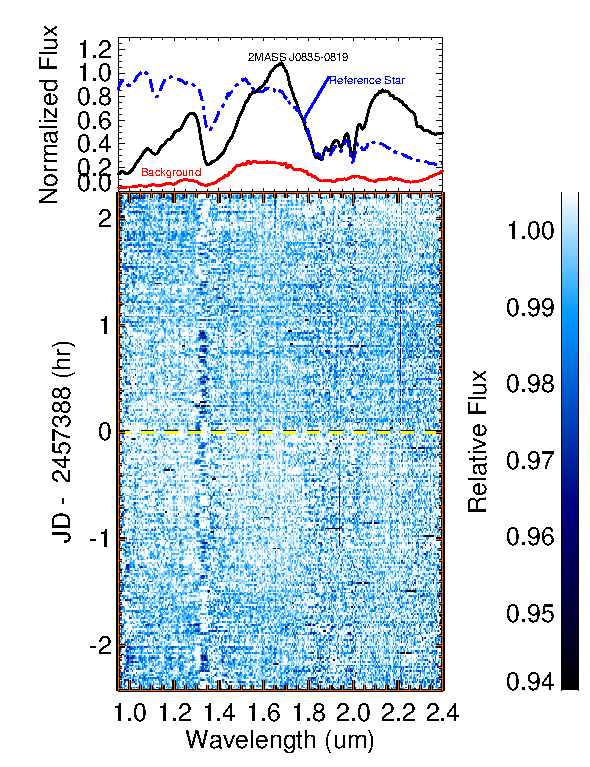
\includegraphics[width=0.5\textwidth]{specphot_j0835.pdf}
	\label{fig:specphot0835}
	}
\subfloat[2MASS J1821]{
	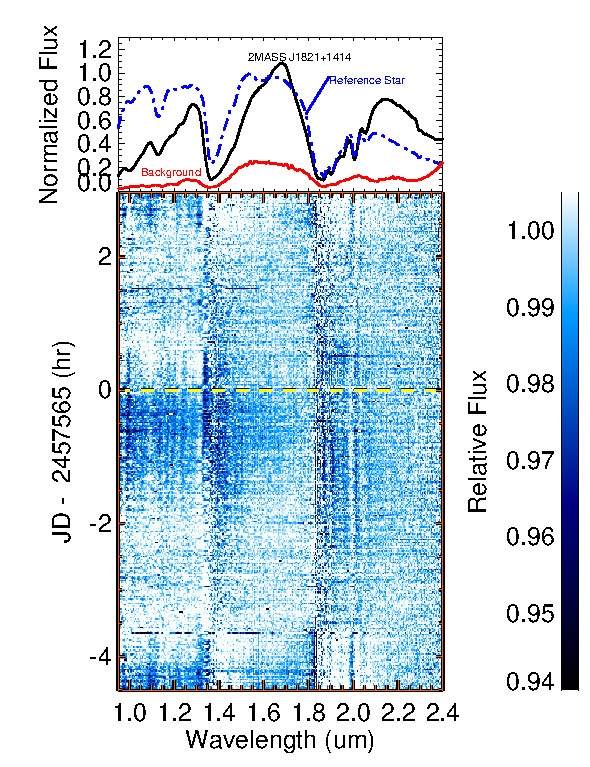
\includegraphics[width=0.5\textwidth]{specphot_j1821.pdf}
	\label{fig:specphot1821}
	}
	\caption{Top Panels: Normalized median raw spectra of {\sha} (left) and {\shb} (right) in black, compared with the respective reference stars (blue) and background emission (red; mostly telluric OH emission and thermal background).  Bottom Panels: Dynamic spectra of each brown dwarf system. The dynamic spectrum for \sha\ shows no significant variability in the spatial or spectral direction whereas \shb\ shows significant repeated modulations with a period near 4 hours.
The variability in \shb\ is prominent at the short wavelengths with a magnitude of ~$\sim$2\% peak-to-trough at short wavelengths but $\lesssim 0.5\%$ toward 2~$\mu$m.}
	\label{fig:specphot}
	\vspace{0.1in}
\end{figure*} 


The images were rectified by shifting each row to match a center row in between the two sources.
This was achieved by cross correlating the reference row with all other detector rows (which have the same background spectrum) and fitting a smooth function over the sources as in \citealt{2016ApJ...826..156S}.
We also obtained calibration sequences of ThAr and flat-field incadescent lamps with the 3$\arcsec$$\times$60$\arcsec$ slit  before and after the brown dwarf time series.
An additional set of ThAr emission lamp spectra were taken at the beginning and end of the observations (preceding and following the 3$\arcsec \times 60 \arcsec$ lamp spectra) with a 0.3$\arcsec\times60\arcsec$ slit for wavelength calibration.
% to measure pixel response and assess flexure in the instrument with telescope orientation.
For {\sha}, we used a combination of the flat-field lamp and a sky frame to construct a pixel response map, removing large-scale ($\gtrsim$ 30 pixels) structure with low order polynomial fits along spatial and spectral axes, and normalizing to the median response. 
To correct for instrument flexure, we also cross-correlated the sky frame with each science image to measure linear spatial shifts, which were $\pm$5~pixels or 0.5\arcsec\ for \sha\ and $\pm$1.5~pixels or 0.15\arcsec\ for \shb.
These shifts were used to apply a custom flat field for every image.
For {\shb}, we did not have sufficient sky frames so we used our incandescent lamp image for both flat fielding and flexure analysis.

As described in \citet{2016ApJ...826..156S}, we performed spatial background subtraction over the entire slit using a 4th-order polynomial fit to points more than 30 pixels away from the center of the source dispersion traces.  Spectra were optimally extracted \citep{1986ApJ...302..757H}, with spatial profiles fit to low order polynomials along the spectral direction one row at a time with 20$\sigma$ rejection to remove cosmic rays and bad pixels.
These spatial profiles were then used to calculate a weighted sum spectrum across the illuminated detector for each source and exposure. 
Typical signals-to-noise of the extracted spectra were 40 - 100 per spectral pixel (unbinned).
Relative spectra (source/reference) were then computed for each exposure.
Our image rectification process described above ensures that the wavelength solution is the same for each row if the image.
However, there are small additional shifts of the sources within the slit so another shift is performed between the sources to ensure the telluric features removed when dividing the two spectra.

%For MORIS reduction, we used the raw files and performed aperture photometry with the IDL \texttt{aper} procedure using an aperture size of 6 pixels and a sky annulus of 8-11 pixels.

\begin{figure*}[!t]
\centering
\subfloat[2MASS J0835]{
	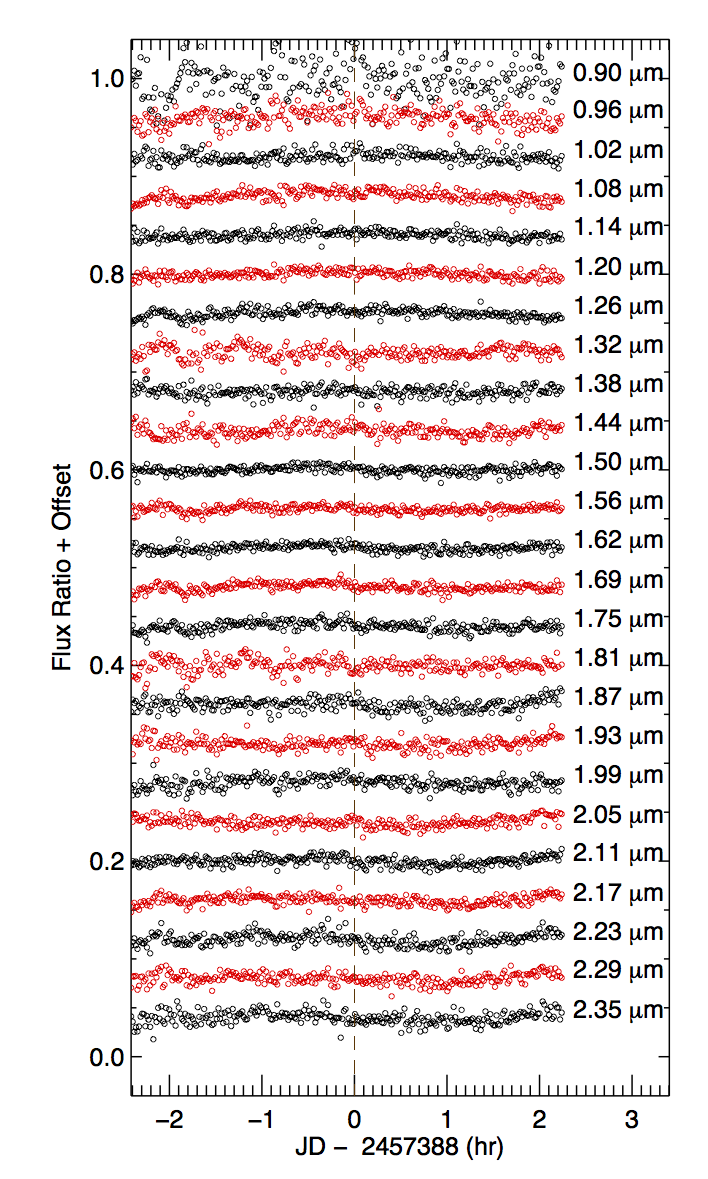
\includegraphics[width=0.5\textwidth]{2mass_0835_t_series.png}
	\label{fig:tserPhase0835}
	}
\subfloat[2MASS J1821]{
	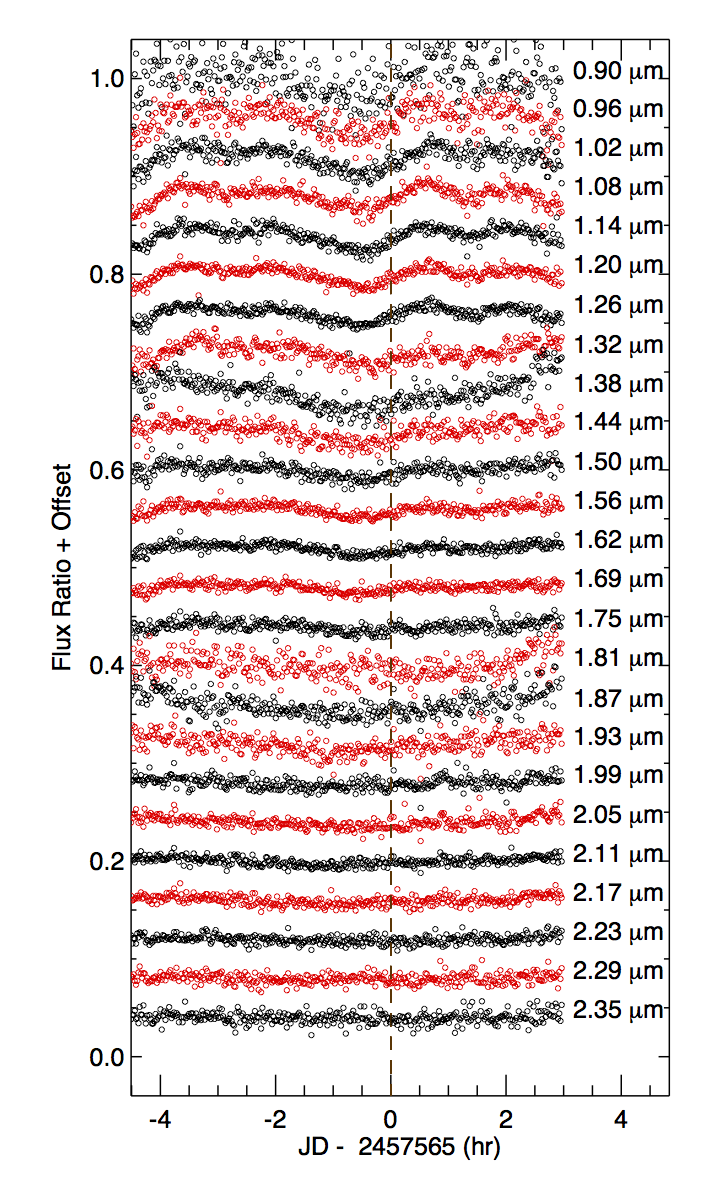
\includegraphics[width=0.5\textwidth]{2mass_1821_t_series.png}
	\label{fig:tserPhase1821}
	}
	\caption{Time series for each system with an offset added for clarity. Each wavelength bin is labeled on the right side. Alternating colors are used to distinguished the light curves with offsets. \sha\ shows relatively flat light curves whereas \shb\ has large amplitude double-peaked oscillations at short wavelengths and flat light curves at long wavelengths.}
	\label{fig:tserPfold}
\end{figure*} 


\begin{figure*}
\centering
\subfloat[2MASS J0835]{
	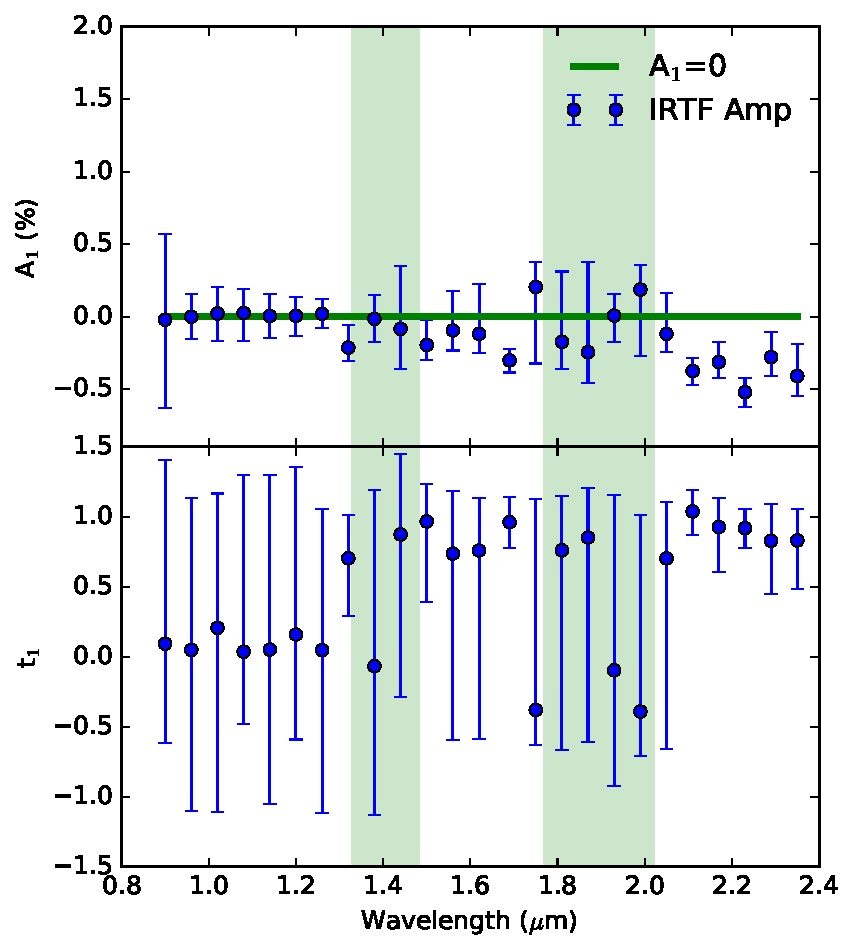
\includegraphics[width=0.5\textwidth]{amp_vs_wavl_j0835.pdf}
	\label{fig:ampspec0835}
	}
\subfloat[2MASS J1821]{
	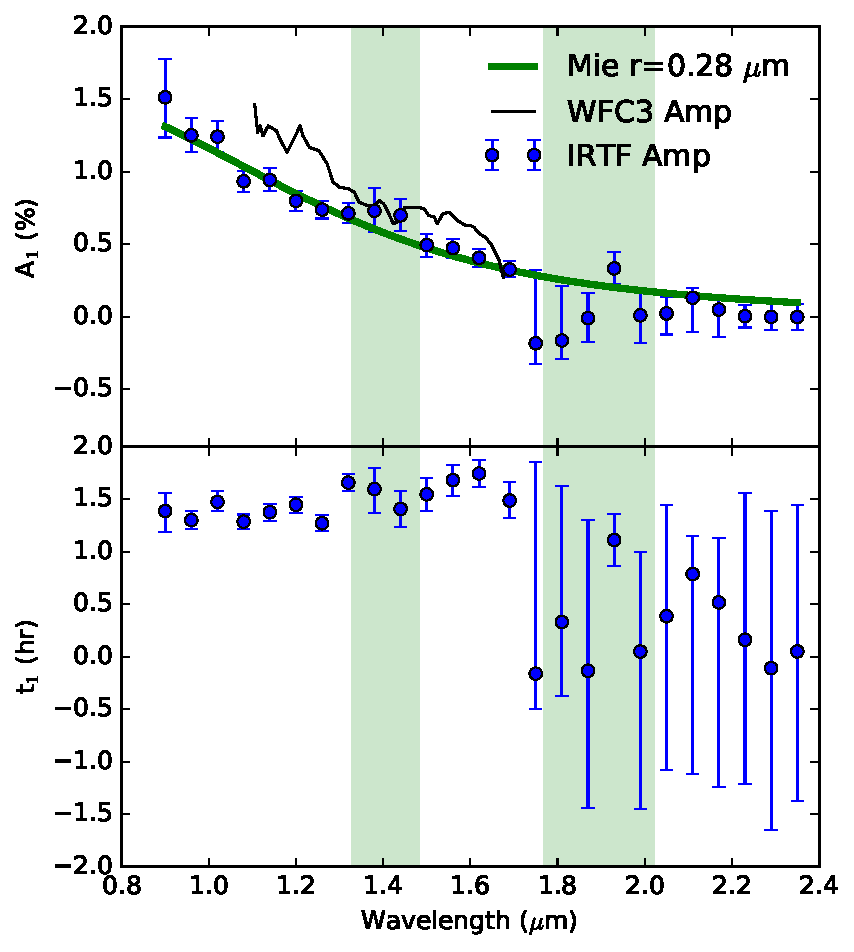
\includegraphics[width=0.5\textwidth]{amp_vs_wavl_j1821.pdf}
	\label{fig:ampspec1821}
	}
	\caption{Sine fit amplitude versus wavelength for each brown dwarf. \sha\ shows no clear trend in wavelength, while \shb\ has a strong slope indicative of Mie-scattering particles.
	 Also shown in the figure for \shb\ is the WFC3 amplitude from \citet{2015ApJ...798L..13Y}. The WFC3 observations were from a different epoch, with different cloud coverage, but show a similar slope.
	 The amplitude spectrum for \shb\ is fit with a simple Mie scattering models for a log-normal particle size distribution of spherical forsterite grains with a best-fit radius of 0.17 $\pm$ 0.01 grains.}
	\label{fig:ampSpec}
\end{figure*} 

\section{Analysis}\label{sec:analysis}

\subsection{Light Curves}

Figure \ref{fig:specphot} shows the raw spectra of the two brown dwarfs, their reference spectra and the background spectra.
Neither the reference spectra nor the brown dwarfs spectra have any corrections applied for telluric absorption or instrumental spectral response.
The reference stars have significantly bluer spectra than the brown dwarfs, but nonetheless contain the same telluric absorption signatures.
The regions near 1.37~$\mu$m and 1.83~$\mu$m have significantly lower flux due to telluric water vapor absorption.

Figure \ref{fig:specphot} also shows the dynamic spectra (relative source brightness as a function of wavelength and time.
{\sha} has a dynamic spectra resembling white noise with no significant variations in either the spectral or spatial direction at the $\lesssim$0.5\% level.
{\shb}, on the other hand, shows a clear periodic signal that is strongest at the shortest wavelengths and declines in amplitude toward the longest wavelengths. The periodic signal is nearly coincident with the 4.2~hr period measured by \citet{2015ApJ...799..154M}, enabling confirmation that the signal is astrophysical rather than systematic (see \citealt{2016ApJ...826..156S}).
Both sources exhibit some systematic features in the strong telluric absorption bands at 1.4 and 1.8~$\mu$m, likely caused by residual wavelength drifts from flexure and lower signals-to-noise.

Individual narrow-band light curves are extracted for each target in 25 spectral bins of width 0.060~$\mu$m; these are shown in Figure~\ref{fig:tserPfold}.
The uncertainties in these curves due to photon and read noise range from 0.2\% to 0.6\% per exposure.
We measure the standard deviations of the time series for wavelength regions that have no significant variations near the rotation period of the brown dwarfs and compare it to the expected photon and read noise.
In these wavelength bins, the standard deviations of the points is about 4$\times$ the expected read noise and photon noise.
We attribute this to correlated errors between wavelengths and as a simple approximation multiply all error bars by a factor of 4 to account for these systematics.

As seen in Figure~\ref{fig:tserPfold}, we see minimal variation in the lightcurves of {\sha}, but pronounced variation in {\shb}, particular in bands $<$1.8~$\mu$m. 
These variations are approximately sinusoidal, although we detect ``double-hump'' structures with slight downturns in flux at peak amplitudes around -2.7~hr and +1.3~hr.
In the regions of strong telluric absorption, the variability pattern changes, with a U-shaped profile minimized at $-$1~hr.
As this pattern aligns with the airmass trend over the sequence of observations, we attribute this pattern to systematic effects and impose priors on the rotational period of the brown dwarfs to ensure the sinusoidal fits do not fit the airmass trend.

Each of the light curves were fit to a simple sinusoidal model:
\begin{equation}\label{eq:cosfit}
F(t) = A \cos(2 \pi (t - t_t)/\tau) + B t + C
\end{equation}
where $F(t)$ is the relative flux as a function of time $t$, $A$ is the amplitude of periodic variations, $t_t$ is the time of maximum periodic flux, $\tau$ is period of the variations, and $B$ and $C$ are linear terms describing any baseline trend.
Since some wavelengths are affected by telluric contamination and we wish to avoid fitting harmonics, we impose a prior on the rotational period $\tau$.
For \sha\ we use a prior 3.0 $< \tau < $3.2 hr from \citet{2004MNRAS.354..378K} and for \shb\ we use 3.8 $< \tau <$ 4.0 hr.
The prior for \shb\ is slightly different from the value from \citet{2015ApJ...799..154M}(4.2 hr) because it came from a fit in a clear region of the time series (at 1.08~$\mu$m) where a double sinusoidal fit resulted in a period of 3.90 $\pm$ 0.01 hr.
Secondly, we restrict the time of maximum periodic flux such that $-\tau/2 < t_1 < \tau/2$ to make sure there are no 2$\pi$ degeneracies in the fit.


Figure \ref{fig:ampSpec} shows the MCMC posterior constraints for periodic amplitudes as a function of wavelength.
For {\sha} (Figure \ref{fig:ampspec0835}) we find small ($\lesssim 0.5\%$) amplitudes with a flat trend as a function of wavelength.
There is low level variability but it is not seen at a constant phase.
\shb, on the other hand, shows a clear decreasing trend as function of wavelength.




The same trend of decreasing variability amplitude for \shb\ was observed by HST's WFC3 grism over a shorter wavelength range (1.1 to 1.7~$\mu$m) by \citet{2015ApJ...798L..13Y}, also shown in Figure \ref{fig:ampspec1821}.
The HST WFC3 maximum over minimum flux spectrum is converted to an amplitude spectrum by assuming that the amplitude is half the difference in maximum and minimum flux, which can be shown to be 
\begin{equation}
A  = \frac{f_R - 1}{f_R + 1}
\end{equation}\label{eq:ampFromRatio}
where $f_R$ is the flux ratio of the maximum over minimum flux.
There is a multiplicative offset between the IRTF and WFC3 spectrum because they were taken at different epochs and therefore different spatial cloud and temperature distributions.
\citet{2015ApJ...798L..13Y} find that the WFC3 spectrum has no significant water vapor absorption which indicates a high haze layer in 2MASS J1821 and is consistent with our gradually decreasing slope from 1.1 to 1.7~$\mu$m.

\subsection{Mie Scattering Fit}

\begin{figure}
\begin{centering}
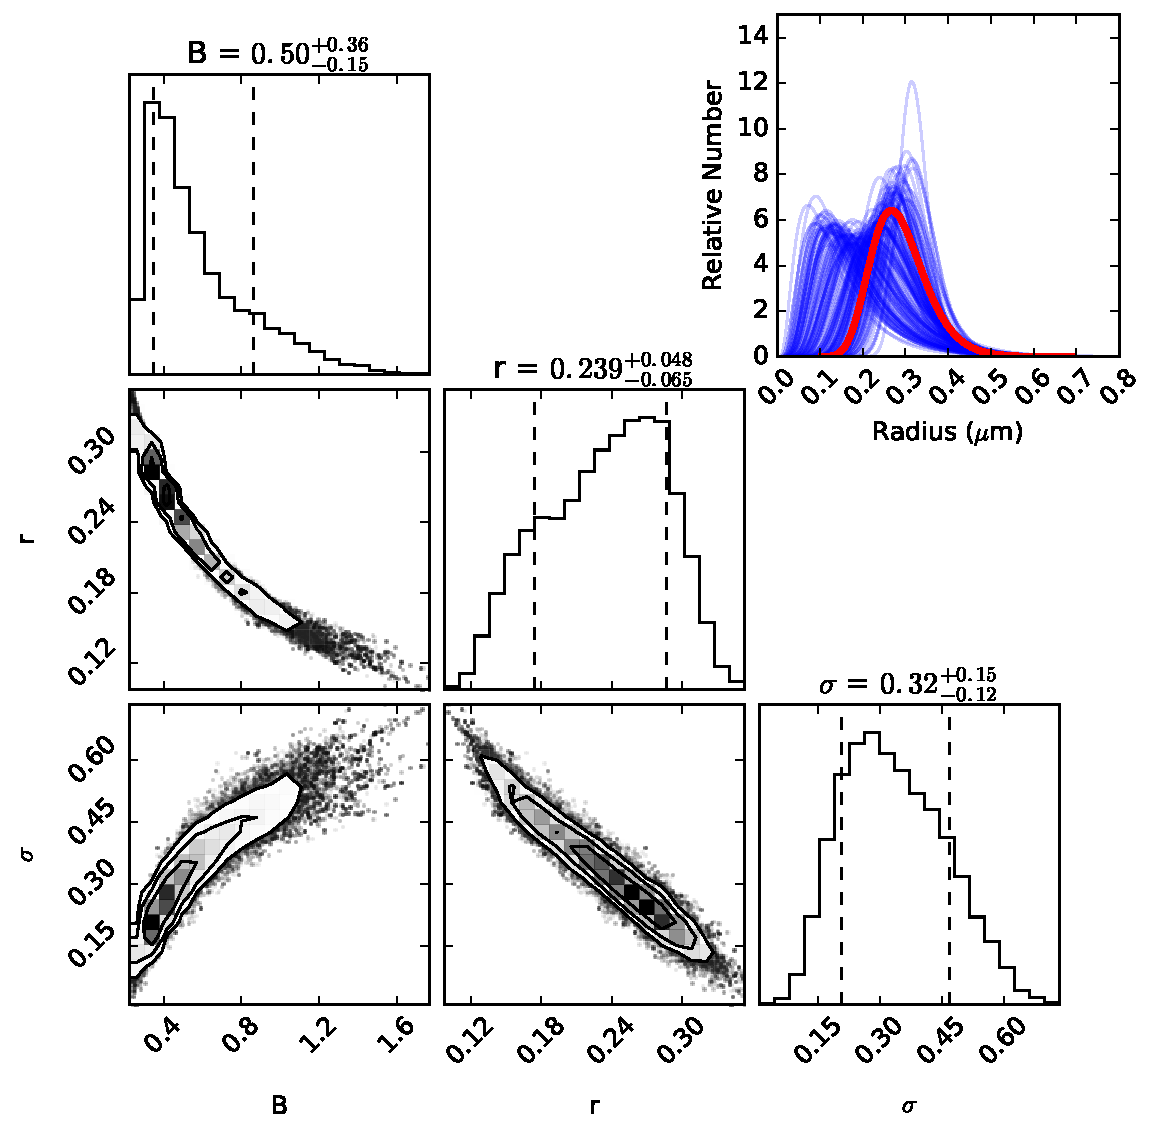
\includegraphics[width=0.5\textwidth]{corner_j1821_mie_sc.pdf}
\caption{Posterior distributions to the simple Mie scattering fit to the amplitude spectrum for \shb.
The model includes an amplitude offset, $B$, (to account for areal coverage) and a median particle radius, $r$.}\label{fig:corner1821mie}
\end{centering}
\end{figure}

We model the wavelength dependence of 2MASS 1821 as an optically thin cloud layer consisting of a log-normal distribution of particle sizes.
If we assume the cloud covers one hemisphere of the brown dwarf, the amplitude of the variability ($A$) is directly proportional to the opacity of the particles.
We model the single particle extinction coefficient, $Q_{ext}$ from the \texttt{Python} Mie theory code \texttt{miescatter} \citep{bohren1983mie} to calculate the opacity as a function of wavelength.
We assume that the particles are spherical forsterite grains (Mg$_2$SiO$_4$).
We use a constant n=1.67 - 0.006 $j$ index of refraction because the real and imaginary parts of the index of refraction are relatively constant across the optical and near infrared \citep{scott1996forsterite}.

For the particle size distribution we assume a log-normal distribution around a characteristic size, $s$ and a standard deviation of the logarithm (scale parameter), $\sigma$ =0.5.
The spectral dependence is therefore modeled as 
\begin{equation}
A = B \bar{Q_{avg}}(r)
\end{equation}
where $A_1$ is the amplitude, $B$ is a constant encapsulating the area and column density and $\bar{Q_{avg}}(r)$ is the average extinction coefficient averaged over all particles in the log-normal distribution with a median radius of $r$.

Figure \ref{fig:ampspec1821} shows the best-fit model which has a median particle radius of 0.16~$\mu$m grains.
This model has a reduced $\chi^2$ of 0.99 and is consistent with the measured amplitude spectrum.
Figure \ref{fig:corner1821mie} shows the posterior distribution for the $B$ and $r$ parameters.
The derived median particle radius of $r$=0.164 $^{+0.012}_{-0.007}$~$\mu$m is a vary tight constraint for particle size median.
Considering the large number of possible grain geometries and compositions, this is an underestimate for the true uncertainty in median particle size.


A similar amplitude versus wavelength trend was recently observed for WISEP J004701.06+680352.1 \citep{2016ApJ...829L..32L}, which has very red ($J-K$ = 2.55) spectral energy distribution thought to be caused by a high altitude haze layer.
In WISEP J0047, the wavelength trend could be fit by $\sim0.4~\mu$m forsterite grains, a few times large than our characteristic particle size.

\subsection{Spot Model Fit}\label{sec:spotModel}

\begin{figure}
\begin{centering}
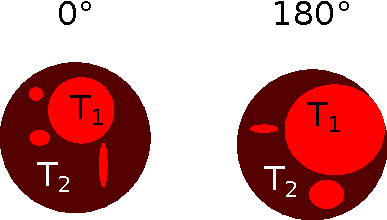
\includegraphics[width=0.4\textwidth]{temperature_drawing.pdf}
\caption{A simple two region model with two different temperatures and different areal fractions for longitudes 0\degree\ and 180\degree.}\label{fig:tdiffschem}
\end{centering}
\end{figure}

Another simple model we attempt assumes  that the brown dwarf spectral variability has to do with a non-uniform temperature distribution on the brown dwarf in the same way that starspots modulate the brightness of hydrogen burning stars as they spin.
In Figure \ref{fig:ampspec1821tdiff}, we fit the same amplitude spectrum as in Figure \ref{fig:ampspec1821}.
This time we model the data with two temperature regions as shown in Figure \ref{fig:tdiffschem}, with two opposite longitudes of the planet at the brightness minimum and maximum.
We assume for the purposes of variability that each hemisphere and layer is in local thermodynamic equilibrium (LTE) so that the flux is proportional to the Planck function times the areal coverage.
The flux ratio between maximum and minimum flux is then
\begin{equation}
f_{R,\lambda} = \frac{\alpha_1 B_\lambda(T_1) + (1-\alpha_1) B_\lambda(T_2)}{\alpha_2 B_\lambda(T_1) + (1-\alpha_2) B_\lambda(T_2)}
\end{equation}
where $\alpha_1$ and $\alpha_2$ are the areal fractions of the first ($T_1$ and second ($T_2$) regions respectively, $B_\lambda$ is the Planck function, and $T_1$ and $T_2$ are the temperatures of the two regions.
$\alpha_1$ and $\alpha_2$ are limited to [0,1].
Using equation \ref{eq:ampFromRatio}, the amplitude then becomes
\begin{equation}\label{eq:twoTempAmpAlphas}
A_\lambda = \frac{\left(\alpha_1 - \alpha_2 \right) \left(B_\lambda(T_1) - B_\lambda(T_2) \right)}{\left(\alpha_1 + \alpha_2\right) B_\lambda(T_1) + \left(2 - \alpha_1 - \alpha_2\right) B_\lambda(T_2)}.
\end{equation}
If the temperature difference is significant so that one Planck function is in the Wien's limit while the other is in the Rayleigh Jeans tail, the cooler temperature essentially becomes black and the contrast approaches a constant for short wavelengths.
If we ignore projection effects for small area coverage, the effective temperature is 
\begin{equation}
\sigma T_{eff}^4 \approx (\alpha_1 + \alpha_2) \sigma T_1^4 + (2 - \alpha_1 - \alpha_2) \sigma T_2^4
\end{equation}
where $\sigma$ is the Stephan-Boltzmann constant.

In the model fitting, we found a strong correlation between $\alpha_1$ and $\alpha_2$.
Therefore we re-parameterized with $\beta = \alpha_1 - \alpha_2$, so that $\alpha_2 = \alpha_1 - \beta$.
\begin{equation}\label{eq:twoTempAmp}
A_\lambda = \frac{\beta \left(B_\lambda(T_1) - B_\lambda(T_2) \right)}{\left(2 \alpha_1 - \beta \right) B_\lambda(T_1) + \left(2 - 2 \alpha_1 + \beta \right) B_\lambda(T_2)}.
\end{equation}

We start by considering a two-faced model where $\alpha_1$ = 1 and $\alpha_2$ = 0, so that the two halves of the brown dwarf are different temperatures.
To be close to the effective temperature of the brown dwarf, we fix $T_1$ to be 1600 K and only vary $T_2$.
This model is a poor match to the data, also shown in Figure \ref{fig:ampspec1821tdiff} with a reduced chi-squared, $\bar{\chi}^2$ = 15.
Next, we attempt a model where we allow $\alpha_1$ and $\alpha_2$ to be free parameters and restrict the temperature limits of the two regions to [1300,2500] to ensure that the final effective temperature is close to the measured 1600 K \citep{gagne2015banyan7}.
The best fit model has $T_{eff} \approx $1590 K and $\bar{\chi}^2$=2.1, but pushes to the edges of our prior with $T_1$ = 2500 K and $T_2$ = 1300 K.
Finally, we consider a model where all four parameters, $\alpha_1$, $\alpha_2$, $T_1$ and $T_2$ are all free.
With these loose constraints, the model fits the data with $\bar{\chi}^2$ = 1.3, consistent with the data, but not with the effective temperature ($T_{eff}$ = 850 K).
The $\alpha$ values are both $<<1$, indicating that the model fits with dark patches on a small fraction of the surface. [I MODIFIED THIS SENTENCE; IS IT CORRECT? I'm a little confused about how both $\alpha$ values can be $<<1$; if one is small doesn't the other have to be large?]

The temperature contrasts in these models (with the exception of the two-faced model which poorly matches the data) are significantly larger than the expected 50 K horizontal temperature variations expected in circulation models \citep{showman2013bdgpDynamics}.
Therefore, we suspect that hot or cold spots on the surface are a less plausible explanation of the variability of 2MASS J1821 than a heterogenous temperature distribution.

\vspace{0.2in}
\begin{figure}
\begin{centering}
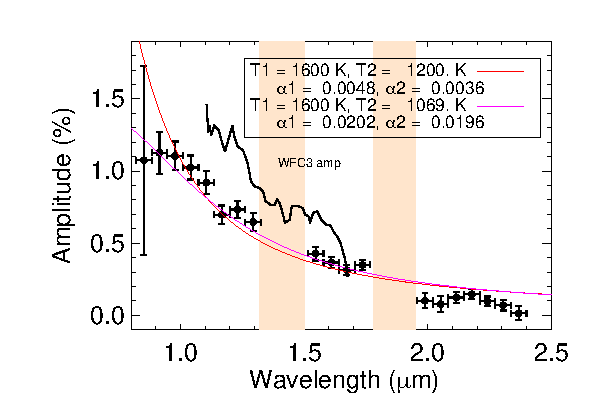
\includegraphics[width=0.5\textwidth]{amp_vs_wavl_j1821_t_diff.pdf}
\caption{The same data as in Figure \ref{fig:ampspec1821}. We fit the data with a two region model that assumes the effective temperature of the brown dwarf and a cooler temperature.}\label{fig:ampspec1821tdiff}
\end{centering}
\end{figure}
% Command used:
% plot_rad_vs_wavl,/amp,/shadetell,custxrange=[0.8,2.5],custyrange=[-0.1,1.9],/showYang,/twoTreg





\section{Conclusions}\label{sec:conclusions}

We observed two brown dwarfs of spectral type L4-L5: 2MASS 1821 and 2MASS 0835.
These brown dwarfs have temperatures near the condensation temperatures of MgSiO$_3$ and Mg$_2$SiO$_4$.
We obtained high precision ground-based spectrophotometry of both systems to measure the variability spectra of these systems with the IRTF.
After fitting sinusoids to both of the time series, we find that 2MASS 0835 has low levels of variability and no significant wavelength dependence.

2MASS J1821 shows significant variability up to the 1.1\% amplitude at short wavelengths (0.8$\mu$m) which decreases towards the near infrared (2.4$\mu$m).
This is consistent with HST measurements for the system that show a gradual decrease in variability amplitude with wavelength \citep{2016ApJ...826....8Y} from 1.1$\mu$m to 1.7 $\mu$m with no decrease in the water vapor band.
The lack of the water vapor band gives evidence of a high altitude aerosol layer in the atmosphere.

We fit the variability amplitude spectrum with an optically thin Mie scattering model and find it is consistent with forsterite (Mg$_2$SiO$_4$) grains with sub-micron sized particles.
A log-normal particle size distribution with a median of 0.2$\mu$m fits the data with a $\bar{\chi^2}$ of 2.5.
We also model the wavelength dependence with a spotted surface model with two different Planck functions covering different spatial regions.
The two temperature region model can fit variability amplitude spectrum well within errors, but gives implausible temperature differences.
Therefore, we favor the Mie scattering model as a better explanation for the variability amplitude spectrum.

\section{Acknowledgements}
MCMC fitting makes use of \texttt{emcee} \citep{foreman-mackey2013emcee} and the covariance plot was made with \texttt{corner.py} \citep{foremanCorner}.
Thanks to Vivien Parmentier for useful discussions on cloud versus a spotted temperature model.
Funding for the E Schlawin is provided by NASA Goddard Spaceflight Center.
This research has made use of the Exoplanet Orbit Database and the Exoplanet Data Explorer at exoplanets.org.
This research made use of the \texttt{astropy} package \citep{astropy2013}. The authors wish to recognize and acknowledge the very significant cultural role and reverence that the summit of Mauna Kea has always had within the indigenous Hawaiian community. We are most fortunate to have the opportunity to conduct observations from this mountain.

%If  used, this work made use of the \texttt{astropy} package \citep{astropy2013}.
%If used, some data was collected from the Open Exoplanet Catalogue \citep{rein2012openExoCat}.

%% In a manner similar to \objectname authors can provide links to dataset
%% hosted at participating data centers via the \dataset{} command.  The
%% second curly bracket argument is printed in the text while the first
%% parentheses argument serves as the valid data set identifier.  Large
%% lists of data set are best provided in a table (see Table 3 for an example).
%% Valid data set identifiers should be obtained from the data center that
%% is currently hosting the data.
%%
%% Note that AASTeX interprets everything between the curly braces in the 
%% macro as regular text, so any special characters, e.g. "#" or "_," must be 
%% preceded by a backslash. Otherwise, you will get a LaTeX error when you 
%% compile your manuscript.  Special characters do not 
%% need to be escaped in the optional, square-bracket argument.



%% In this section, we use  the \subsection command to set off
%% a subsection.  \footnote is used to insert a footnote to the text.

%% Observe the use of the LaTeX \label
%% command after the \subsection to give a symbolic KEY to the
%% subsection for cross-referencing in a \ref command.
%% You can use LaTeX's \ref and \label commands to keep track of
%% cross-references to sections, equations, tables, and figures.
%% That way, if you change the order of any elements, LaTeX will
%% automatically renumber them.

%% This section also includes several of the displayed math environments
%% mentioned in the Author Guide.


%% The equation environment wil produce a numbered display equation.


%% The \notetoeditor{TEXT} command allows the author to communicate
%% information to the copy editor.  This information will appear as a
%% footnote on the printed copy for the manuscript style file.  Nothing will
%% appear on the printed copy if the preprint or
%% preprint2 style files are used.

%% The eqnarray environment produces multi-line display math. The end of
%% each line is marked with a \\. Lines will be numbered unless the \\
%% is preceded by a \nonumber command.
%% Alignment points are marked by ampersands (&). There should be two
%% ampersands (&) per line.

%% Putting eqnarrays or equations inside the mathletters environment groups
%% the enclosed equations by letter. For instance, the eqnarray below, instead
%% of being numbered, say, (4) and (5), would be numbered (4a) and (4b).
%% LaTeX the paper and look at the output to see the results.

%% This section contains more display math examples, including unnumbered
%% equations (displaymath environment). The last paragraph includes some
%% examples of in-line math featuring a couple of the AASTeX symbol macros.

%% The displaymath environment will produce the same sort of equation as
%% the equation environment, except that the equation will not be numbered
%% by LaTeX.
%% If you wish to include an acknowledgments section in your paper,
%% separate it off from the body of the text using the \acknowledgments
%% command.

%% Included in this acknowledgments section are examples of the
%% AASTeX hypertext markup commands. Use \url without the optional [HREF]
%% argument when you want to print the url directly in the text. Otherwise,
%% use either \url or \anchor, with the HREF as the first argument and the
%% text to be printed in the second.

\acknowledgments



%% To help institutions obtain information on the effectiveness of their
%% telescopes, the AAS Journals has created a group of keywords for telescope
%% facilities. A common set of keywords will make these types of searches
%% significantly easier and more accurate. In addition, they will also be
%% useful in linking papers together which utilize the same telescopes
%% within the framework of the National Virtual Observatory.
%% See the AASTeX Web site at http://aastex.aas.org/
%% for information on obtaining the facility keywords.

%% After the acknowledgments section, use the following syntax and the
%% \facility{} macro to list the keywords of facilities used in the research
%% for the paper.  Each keyword will be checked against the master list during
%% copy editing.  Individual instruments or configurations can be provided 
%% in parentheses, after the keyword, but they will not be verified.

%{\it Facilities:} \facility{Nickel}, \facility{HST (STIS)}, \facility{CXO (ASIS)}.

%% Appendix material should be preceded with a single \appendix command.
%% There should be a \section command for each appendix. Mark appendix
%% subsections with the same markup you use in the main body of the paper.

%% Each Appendix (indicated with \section) will be lettered A, B, C, etc.
%% The equation counter will reset when it encounters the \appendix
%% command and will number appendix equations (A1), (A2), etc.

%\appendix


%% The reference list follows the main body and any appendices.
%% Use LaTeX's thebibliography environment to mark up your reference list.
%% Note \begin{thebibliography} is followed by an empty set of
%% curly braces.  If you forget this, LaTeX will generate the error
%% "Perhaps a missing \item?".
%%
%% thebibliography produces citations in the text using \bibitem-\cite
%% cross-referencing. Each reference is preceded by a
%% \bibitem command that defines in curly braces the KEY that corresponds
%% to the KEY in the \cite commands (see the first section above).
%% Make sure that you provide a unique KEY for every \bibitem or else the
%% paper will not LaTeX. The square brackets should contain
%% the citation text that LaTeX will insert in
%% place of the \cite commands.

%% We have used macros to produce journal name abbreviations.
%% AASTeX provides a number of these for the more frequently-cited journals.
%% See the Author Guide for a list of them.

%% Note that the style of the \bibitem labels (in []) is slightly
%% different from previous examples.  The natbib system solves a host
%% of citation expression problems, but it is necessary to clearly
%% delimit the year from the author name used in the citation.
%% See the natbib documentation for more details and options.

\bibliographystyle{apj}
\bibliography{bd_biblio}

%\clearpage

%% Use the figure environment and \plotone or \plottwo to include
%% figures and captions in your electronic submission.
%% To embed the sample graphics in
%% the file, uncomment the \plotone, \plottwo, and
%% \includegraphics commands
%%
%% If you need a layout that cannot be achieved with \plotone or
%% \plottwo, you can invoke the graphicx package directly with the
%% \includegraphics command or use \plotfiddle. For more information,
%% please see the tutorial on "Using Electronic Art with AASTeX" in the
%% documentation section at the AASTeX Web site, http://aastex.aas.org/
%%
%% The examples below also include sample markup for submission of
%% supplemental electronic materials. As always, be sure to check
%% the instructions to authors for the journal you are submitting to
%% for specific submissions guidelines as they vary from
%% journal to journal.

%% This example uses \plotone to include an EPS file scaled to
%% 80% of its natural size with \epsscale. Its caption
%% has been written to indicate that additional figure parts will be
%% available in the electronic journal.

%\begin{figure}
%\epsscale{.80}
%\plotone{f1.eps}
%\caption{Derived spectra for 3C138 \citep[see][]{heiles03}. Plots for all sources are available
%in the electronic edition of {\it The Astrophysical Journal}.\label{fig1}}
%\end{figure}

%\clearpage

%% Here we use \plottwo to present two versions of the same figure,
%% one in black and white for print the other in RGB color
%% for online presentation. Note that the caption indicates
%% that a color version of the figure will be available online.
%%

%\begin{figure}
%\plottwo{f2.eps}{f2_color.eps}
%\caption{A panel taken from Figure 2 of \citet{rudnick03}. 
%See the electronic edition of the Journal for a color version 
%of this figure.\label{fig2}}
%\end{figure}

%% This figure uses \includegraphics to scale and rotate the still frame
%% for an mpeg animation.

%\begin{figure}
%\includegraphics[angle=90,scale=.50]{f3.eps}
%\caption{Animation still frame taken from \citet{kim03}.
%This figure is also available as an mpeg
%animation in the electronic edition of the
%{\it Astrophysical Journal}.}
%\end{figure}

%% If you are not including electonic art with your submission, you may
%% mark up your captions using the \figcaption command. See the
%% User Guide for details.
%%
%% No more than seven \figcaption commands are allowed per page,
%% so if you have more than seven captions, insert a \clearpage
%% after every seventh one.

%% Tables should be submitted one per page, so put a \clearpage before
%% each one.

%% Two options are available to the author for producing tables:  the
%% deluxetable environment provided by the AASTeX package or the LaTeX
%% table environment.  Use of deluxetable is preferred.
%%

%% Three table samples follow, two marked up in the deluxetable environment,
%% one marked up as a LaTeX table.

%% In this first example, note that the \tabletypesize{}
%% command has been used to reduce the font size of the table.
%% We also use the \rotate command to rotate the table to
%% landscape orientation since it is very wide even at the
%% reduced font size.
%%
%% Note also that the \label command needs to be placed
%% inside the \tablecaption.

%% This table also includes a table comment indicating that the full
%% version will be available in machine-readable format in the electronic
%% edition.

%% If you use the table environment, please indicate horizontal rules using
%% \tableline, not \hline.
%% Do not put multiple tabular environments within a single table.
%% The optional \label should appear inside the \caption command.



%% If the table is more than one page long, the width of the table can vary
%% from page to page when the default \tablewidth is used, as below.  The
%% individual table widths for each page will be written to the log file; a
%% maximum tablewidth for the table can be computed from these values.
%% The \tablewidth argument can then be reset and the file reprocessed, so
%% that the table is of uniform width throughout. Try getting the widths
%% from the log file and changing the \tablewidth parameter to see how
%% adjusting this value affects table formatting.

%% The \dataset{} macro has also been applied to a few of the objects to
%% show how many observations can be tagged in a table.


%% Tables may also be prepared as separate files. See the accompanying
%% sample file table.tex for an example of an external table file.
%% To include an external file in your main document, use the \input
%% command. Uncomment the line below to include table.tex in this
%% sample file. (Note that you will need to comment out the \documentclass,
%% \begin{document}, and \end{document} commands from table.tex if you want
%% to include it in this document.)

%% \input{table}

%% The following command ends your manuscript. LaTeX will ignore any text
%% that appears after it.

\end{document}

%%
%% End of file `sample.tex'.
